\chapter{Methods}

\section{Fathi Rabbani / 1164074}
\subsection{Teori}
\begin{enumerate}
\item Random Forest
\subitem
Random forest  adalah suatu algoritma yang digunakan pada klasifikasi data dalam jumlah yang besar. Klasifikasi random forest dilakukan melalui penggabungan pohon (tree) dengan melakukan training pada sampel data yang dimiliki. Penggunaan pohon (tree) yang semakin banyak akan mempengaruhi akurasi yang akan didapatkan menjadi lebih baik. Penentuan klasifikasi dengan random forest diambil berdasarkan hasil voting dari tree yang terbentuk. Pemenang dari tree yang terbentuk ditentukan dengan vote terbanyak. berikut adalah struktur dari Random Forest ada pada Gambar \ref{fig1}

\item Membaca Dataset, Makna setiap file dan Menjelaskan data CUB-200-2011
\begin{enumerate}
\item Membaca Data
\begin{itemize}
\item
dengan membuka data yang sudah didownload yaitu data CUB-200-2011 atau data tentang perbandingan data jenis burung,
\item
lalu data tersebut dibuka dengan menggunakan aplikasi Spyder, dan dijalankan setiap baris Code yang ada.
\item data yang ada pada folder CUB-200-2011 dibuka dengan menggunakan code dari Chapter 2 yang ada pada buku pembelajaran.
\end{itemize}

\item Makna setiap File
\begin{itemize}
\item data yang terdapat pada file CUB-200-2011 ada data folder ATTRIBUTE, IMAGES, PARTS yang memiliki kegunaannya sendiri yang dimana pada penggunaannya data yang dipakai adalah data image\_attribute\_label pada folder attribute, data image\_class\_labels dan data classes.
\item file image\_attribute\_label berguna sebagai data awal yang digunakan untuk membaca data attribute yang terdapat pada masing - masing gambar burung yang ada.
\item sedangkan file image\_class\_label yang ada pada folder CUB-200-2011 berguna sebagai data yang akan membuat kolom baru pada dataset yang fungsinya adalah untuk memasukan hasil dari semua data yang dimiliki oleh imgatt2.
\item dan file classes berguna sebagai dataset yang akan dipanggil oleh fungsi code untuk menampilkan nama dari data burung yang dimiliki.
\end{itemize}

\item Isi Field
\begin{itemize}
\item file image\_attribute\_label
berisi tentang data attribute yang ada pada data gambar file burung yang dimiliki difolder image pada CUB-200-2011
\item file image\_class\_label
berisi tentang data yang dimiliki oleh attribute dari image\_attribute\_label dimana data yang bernilai atau memiliki nilai disusun hingga menghasilkan data yang mudah dipahami.
\item file classes
berisi tentang data yang berguna untuk menampilkan data nama dari setiap data jenis burung yang dimiliki.
\end{itemize}
\end{enumerate}

\item Cross Validation
\subitem
Cross-validation adalah metode statistik yang dapat digunakan untuk mengevaluasi kinerja model atau algoritma dimana data dipisahkan menjadi dua subset yaitu data training dan data testing.

\item Score 44 Random Forest, 27 Decision Tree dan 29 SVM
\begin{enumerate}
\item
merupakan hasil dari pengolahan tentang data jenis burung yang dimiliki setelah melalui proses pembagian data training dan testing yang menghasilkan score 44 persen sebagai pembanding bahwa data yang diolah tersebut bernilai 44 persen tingkat kebenarannya atau keakuratannya.
\item
lalu pada penggunaan decision tree yang menghasilkan nilai 27 persen menjelaskan bahwa data yang diolah dengan menggunakan decision tree sebagai fungsi pembandingannya itu lebih kecil tingkat keakuratan hasilnya yang dimana kita mencari keakuratan data dari setiap jenis burung yang ada.
\item
sedangkan dengan menggunakan SVM menghasilkan nilai sebesar 29 persen yang dimana merupakan nilai nertal menjelaskan bahwa data yang diolah masih belum akurat tingkat kesamaannya dengan data jenis burung yang dimiliki.
\end{enumerate}
dari penjelasan tersebut disimpulkan bahwa penggunaan randowm forest dalam menentukan keakuratan data itu lebih besar scorenya dibandingkan menggunakan decision tree dan SVM.

\item Membaca Confusion Matriks
\begin{verbatim}
import numpy as np
np.set_printoptions(precision=2)
plt.figure(figsize=(60,60), dpi=300)
plot_confusion_matrix(cm, classes=birds, normalize=True)
plt.show()
\end{verbatim}
penggunaan code diatas adala cara untuk membaca dataset jenis burung dengan metode confusion matriks. dimana contoh hasil dari membaca data dengan menggunakan confusion matriks adalah sebagai berikut : Gambar \ref{fig2}

\item Voting pada Random Forest
voting pada random forest berguna untuk mengambil nilai yang akan digunakan sebagai bandingan dari masing - masing tree yang ada untuk menghasilkan nilai final sebagai data yang diinginkan, contohnya adalah seperti berikut ini : Gambar \ref{fig3}
\end{enumerate}








\section{Cokro Edi Prawiro / 1164069}

\subsection{Teori}
\begin{enumerate}
\item Jelaskan apa itu random forest, sertakan gambar ilustrasi buatan sendiri.\par
Random Forest atau hutan acak yaitu kumpulan dari pohon-pohon keputusan yang digunakan untuk membaca objek tertentu yang telah di sepakati untuk di baca dalam AI. pohon-pohon keputusan tersebut akan memunculkan hasil-hasil yang akan disimpulkan oleh random forest. pembagian jumlah data yang dimasukan kedalam decision tree pada random forest akan di bagi sama rata sesuai codingan atau ketentuan tertentu yang di sepakati. misalkan data yang akan digunakan sebanyak 314 jika dalam satu decision tree di putuskan untuk memiliki 50 data maka pada satu random forest akan terdapat enam atau tujuh decision tree. untuk lebih jelasnya dapat dilihat pemisalan pada gambar \ref{c36} random forest berikut.


\item Jelaskan cara membaca dataset khusus dan artikan makna setiap file dan isi field masing masing file.
langkah pertama download terlebih dahulu dataset nya kemudian buka menggunakan spyder bawaan anaconda untuk mengetahui isi dari dataset tersebut. biasanya data tersebut berisi databerekstensi .txt yang di dalammya terdapat class dari field atau data data yang ada data tersebut. contoh pada data burung ada field index dan angka, index biasanya berisi angka, angka angka tersebut memiliki makna yaitu pengganti nama atau jenis dari burung tersebut sedangkan pada field yang berisi nilai 0 dan 1 berarti menyatakan atau maknanya yaitu memberikan nilai ya dan tidak nilai tersebut di ubah menjadi angka nol dan satu karna data pada field tersebut harus berisi nilai boolean atau pilihan ya dan tidak di karenakan komputer susah membaca nilai dan tidak maka di ubahlah menjadi 0 dan 1 dengan 0 bernilai tidak dan 1 bernilai ya.

\item Jelaskan apa itu Cross Validation.
Cross Validation merupakan cara untuk mengevaluasi hasil dari sebuah metode yang telah digunakan dengan cara membagi dua bagian dari dataset menjadi data training dan data testing kemudian data tersebut diolah hingga muncul tingkat akurasi dari metode yang digunakan contoh pada metode random forest dataset nya di bagi menjadi dua menjadi data training dan data testing kemudian data tersebut di olah oleh mesin untuk melihat tingkat akurasinya maka akan muncul misalkan akurasi kebenaran sebesar 44 \% begitu pula dengan menggunakan metode-metode yang lain seperti decision tree dan SVM.


\item Jelaskan apa arti score 44 \% pada random forest, 27 \% pada decision tree dan 29 \% dari SVM.
maksud dari score 44 \% tersebut yaitu nilai ketepatan atau kebenaran atau bisa disebut hasil dari random forest misalkan dengan metode random forest mesin membaca objek burung, mesin tersebut bisa menyatakan jenis burung tersebut dengan akurasi kebenaran 44 \%. sedangkan pada metode decision tree yaitu 27 \% yang berarti menunjukan bahwa tingkat akurasi ketepatan mesin jika mengerjakan sesuatu atau menyatakan keputusan dengan metode decision tree maka nilai kebenarannya bernilai 27 \%. sedangkan dengan menggunakan metode SVM menunjukan hasil 29 \% yang berarti nilai ketepatan atau kebenaran dalam memecahkan masalah menggunakan metode SVM ini sebesar 29 \% . maka dari itu dapat di simpulkan bahwa dengan menggunakan metode random forest mesin dapat memecahkan masalah lebih akurat dibandingkan dengan menggunakan decision tree dan SVM.


\item Jelaskan bagaimana cara membaca confusion matriks dan contohnya memakai gambar atau ilustrasi sendiri.
cara membaca confusioo matrix dengan cara memasukan para meter nilai yang ada pada datasets contoh pada dataset terdapat class yang disandingkan dengan nama burung untuk di normalisasi maka akan menunjukan nilai matrix yang mendekati nilai benar dalam bentuk angka misalkan 0,5 0,2 dan seterusnya mendekati nilai satu. di karenakan susahnya membaca nilai angka maka sering di ubah menjadi bentuk grafik. dapat di lihat pada gambar \ref{c38}


\item Jelaskan apa itu voting pada random forest disertai dengan ilustrasi gambar sendiri.\par
Voting merupakan data hasil dari decision tree yang terdapat pada random forest. Dimana hasil data tersebut di gunakan sebagai acuan untuk hasil dari random forest. sebagai contoh misalkan pada satu random forest terdapat enam decision tree untuk menentukan jenis pekerjaan orang, pada decision tree ke satu menyimpulkan bahwa pekerjaanya yaitu dosen , pada decision tree ke dua yaitu dosen kemudian pada decision tiga dosen , pada decision tree ke empat yaitu pekerja kantoran, pada decision tree ke lima yaitu pekerja kantoran dan pada decision tree ke enam yaitu dosen. maka pada random forest dapat menyimpulkan hasilnya yaitu dosen. untuk lebih jelasnya dapat dilihat pada gambar \ref{c37} . 

\end{enumerate}

\section{Ahmad Syafrizal Huda / 1164062}
\subsection{Teori}
\begin{enumerate}
\item Random forest ialah sekumpulan classifier yang terdiri dari banyak pohon keputusan dan mengerjakan klasifikasi berdasarkan keluaran dari hasil klasifikasi setiap pohon keputusan anggota. Klasifikasi random forest dikerjakan melalui penggabungan pohon (tree) dengan melakukan training pada sampel data yang dimiliki. Contoh ilustrasi gambar random forest pada gambar \ref{h1}.
\item Cara membaca dataset kasus dan makna setiap file dan isi field masing-masing file
\subitem Gunakan librari pandas yang sudah di install sebelumnya pada python untuk dapat membaca dataset dengan format text file.
\subitem  Selanjutnya buatlah variabel baru misalkan diberi nama dataset yang berisikan perintah untuk membaca file csv.
\begin{verbatim}
import pandas as data
dataset = data.read_csv("car.txt")
dataset.head()
\end{verbatim}
\subitem Pada perintah diatas yaitu memanggil library pandas untuk membaca dataset, membuat variabel dataset yang berisikan data.read\_csv untuk membaca dataset. Pada contoh ini menggunakan txt tapi tetap bisa membaca datasetnya, karena pada saat dijalankan librari pandas secara otomatis akan mengubah data dalam bentuk text file ke format csv. Hasilnya seperti pada gambar \ref{h2}.
\subitem Penjelasan dari isi field pada hasil gambar \ref{h2} yaitu: Atribut Index merupakan atribut otomatis untuk penomoran data yang sudah ada, Atribut Buying merupakan harga beli dari mobil tersebut. dengan value : v high/Sangat mahal,high/mahal,med/Cukup, low/Murah, Atribut Maint merupakan harga perawatan dari mobil tersebut, dengan value sama seperti pada atribut Buying, Atribut Doors merupakan jumlah pintu yang terdapat pada mobil, dengan value 2,3,4,5 more atau lebih dari 5, Atribut Persons merupakan kapasitas orang yang bisa masuk kedapalm mobil, dengan value 2,4, more /lebih, Atribut Lug Boot merupakan ukuran bagasi boot mobil, dengan value small,med,big, Atribut Safety merupakan perkiraan keselamatan mobil, dengan value low,med,high, Yang terakhir yaitu Value, yang dimana merupakan merupakan Class nya atau disebut dengan targetnya menyatakan apakah mobil tersebut dapat diterima atau tidak dan apakah mobil tersebut bagus atau tidak, dengan value unacc, acc, good,v good.
\item Cross validation adalah teknik validasi model untuk menilai bagaimana hasil analisis statistik (model) akan digeneralisasi ke kumpulan data independen. Ini terutama digunakan dalam pengaturan di mana tujuannya adalah prediksi, dan orang ingin memperkirakan seberapa akurat model prediksi akan dilakukan dalam praktek.
\item Arti score 44\% pada random forest yaitu merupakan outputannya untuk hutan acak, arti score 27\% pada decission tree adalah presentasi hasil dari perhitungan dataset acak, dan arti score 29\% dari SVM adalah hasil pendekatan jaringan saraf.  Hasil tersebut didapat dari hasil valdasi silang untuk memastikan bahwa membagi training test dengan cara yang berbeda. Jadi 44\% untuk random forest, 27\% untuk pohon keputusan, dan 29\% untuk SVM. Itu merupakan presentase keakurasian prediksi yang dilakukan pada saat testing menggunakan label pada dataset yang digunakan. Score mendefinisikan aturan evaluasi model.
\item Perhitungan confusion Matriks dapat dilakukan sebagai berikut:
\subitem Import librari Pandas, Matplotlib, dan Numpy.
\subitem Buat variabel x\_aktu yang berisikan data aktual.
\subitem Buat variabel x\_diksi berisikan data yang akan dijadikan sebagai prediksi.
\subitem Buat variabel ak\_confusion yang berisikan crosstab untuk membangun tabel tabulasi silang yang dapat menunjukkan frekuensi kemunculan kelompok data tertentu.
\subitem Pada variabel ak\_confusion definisikan lagi nama baris yaitu Aktual dan kolomnya Prediksi
\subitem Kemudian definisikan suatu fungsi yang diberi nama plot confusion matrix yang berisikan pendefinisian confusion matrix dan juga akan di plotting. untuk code perintah lengkapnya sebagai berikut :
\subitem
\begin{verbatim}
import numpy as cm1
import matplotlib.pyplot as plt
import pandas as cm2
x_aktu = cm2.Series([3, 1, 3, 3, 1, 2, 2, 3, 3, 1, 2, 3], name='Aktual')
x_diksi = cm2.Series([1, 1, 3, 2, 1, 3, 2, 1, 3, 1, 3, 3], name='Prediksi')
ak_confusion = cm2.crosstab(x_aktu, x_diksi)
ak_confusion = cm2.crosstab(x_aktu, x_diksi, rownames=['Aktual'], colnames=['Prediksi'], margins=True)
def plot_confusion_matrix(df_confusion, title='Confusion matrix', cmap=plt.cm.gray_r):
    plt.matshow(ak_confusion, cmap=cmap) # imshow
    #plt.title(title)
    plt.colorbar()
    tick_marks = cm1.arange(len(ak_confusion.columns))
    plt.xticks(tick_marks, ak_confusion.columns, rotation=45)
    plt.yticks(tick_marks, ak_confusion.index)
    #plt.tight_layout()
    plt.ylabel(ak_confusion.index.name)
    plt.xlabel(ak_confusion.columns.name)
plot_confusion_matrix(ak_confusion)
plt.show()
\end{verbatim}
Hasilnya akan seperti pada gambar \ref{h3} :
\item Voting pada random forest sebagaimana voting yaitu suara/hasil untuk setiap target yang diprediksi pada saat melakukan Random Forest. Pertimbangkan target prediksi dengan voting terbanyak/tertinggi sebagai prediksi akhir dari algoritma random forest. Contoh ilustrasi dapat dilihat pada gambar \ref{h4}.
\end{enumerate}

\begin{figure}[ht]
	\centerline{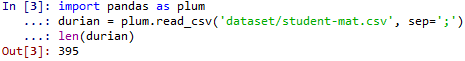
\includegraphics[width=1\textwidth]{figures/fathi/chapter3/1.png}}
	\caption{Random Forest}
	\label{fig1}
\end{figure}

\begin{figure}[ht]
	\centerline{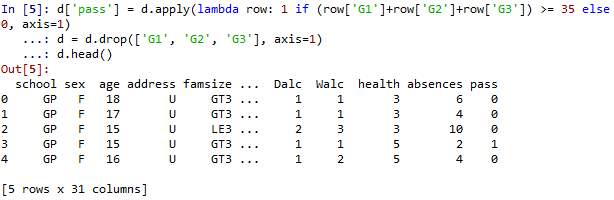
\includegraphics[width=1\textwidth]{figures/fathi/chapter3/2.PNG}}
	\caption{Hasil dari membaca data dengan Confusion Matriks}
	\label{fig2}
\end{figure}

\begin{figure}[ht]
	\centerline{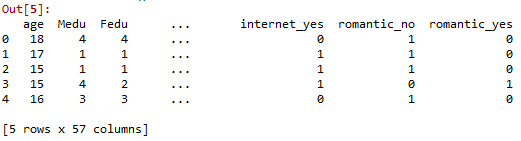
\includegraphics[width=1\textwidth]{figures/fathi/chapter3/3.png}}
	\caption{Voting Random Forest}
	\label{fig3}
\end{figure}




\begin{figure}[ht]
      \centerline{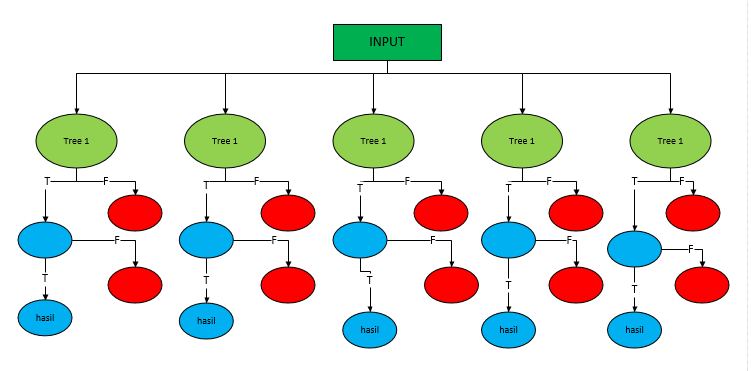
\includegraphics[width=1\textwidth]
      {figures/cokro/c36}}
      \caption{Random Forest}
      \label{c36}
      \end{figure}

\begin{figure}[ht]
      \centerline{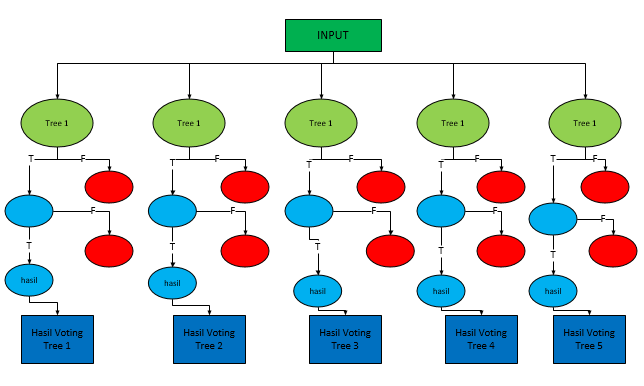
\includegraphics[width=1\textwidth]
      {figures/cokro/c37}}
      \caption{Ilustrasi Voting}
      \label{c37}
      \end{figure}

\begin{figure}[ht]
      \centerline{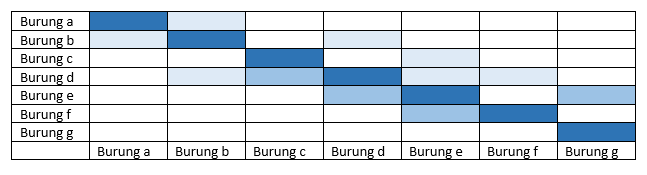
\includegraphics[width=1\textwidth]
      {figures/cokro/c38}}
      \caption{Ilustrasi Confusion matrix}
      \label{c38}
      \end{figure}


\begin{figure}[ht]
	\centerline{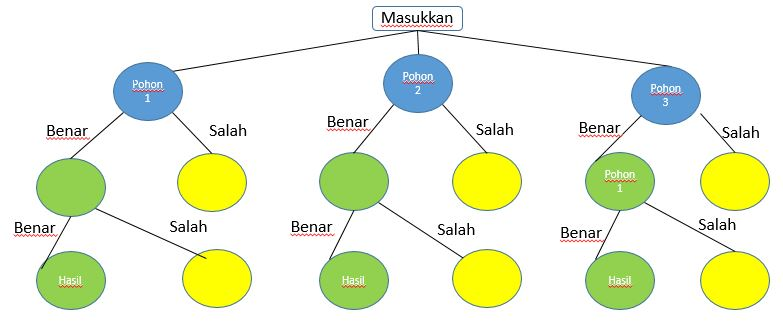
\includegraphics[width=1\textwidth]{figures/huda/chapter3/1.JPG}}
	\caption{Random Forest}
	\label{h1}
\end{figure}

\begin{figure}[ht]
	\centerline{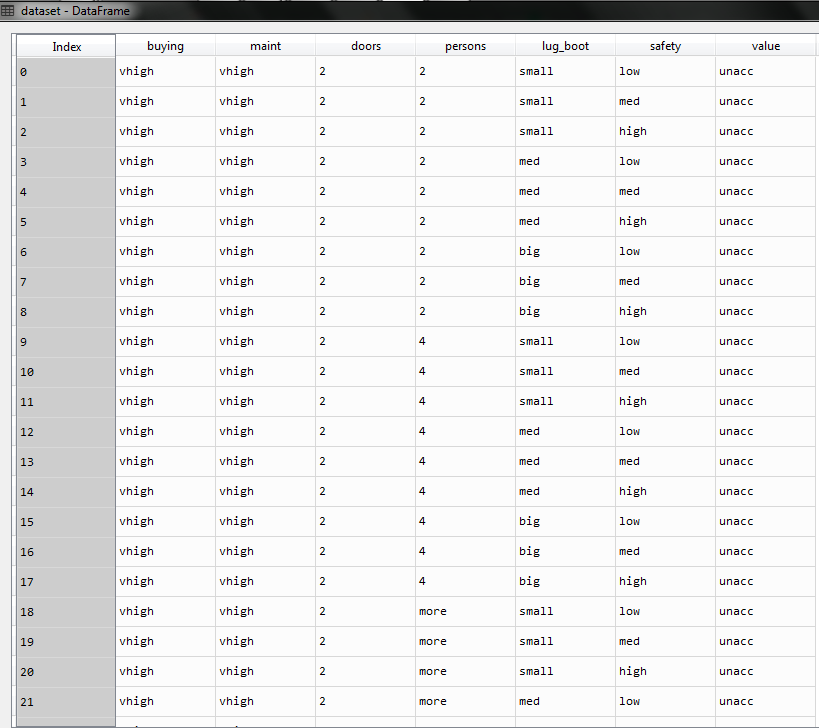
\includegraphics[width=1\textwidth]{figures/huda/chapter3/2.PNG}}
	\caption{Hasil Dataset}
	\label{h2}
\end{figure}

\begin{figure}[ht]
	\centerline{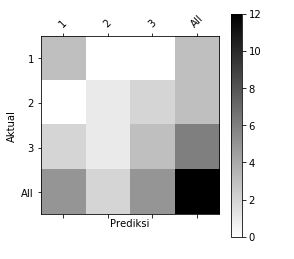
\includegraphics[width=1\textwidth]{figures/huda/chapter3/3.JPG}}
	\caption{Confusion Matrix}
	\label{h3}
\end{figure}

\begin{figure}[ht]
	\centerline{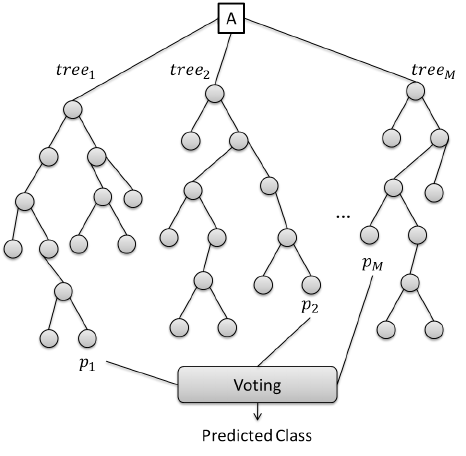
\includegraphics[width=1\textwidth]{figures/huda/chapter3/4.png}}
	\caption{Voting}
	\label{h4}
\end{figure}

